\documentclass[]{beamer}
\usetheme{KUL}
\usepackage{multirow}
\usepackage{multicol}
\usepackage{tikz}
\usepackage{ulem}
\usepackage{siunitx}
\newcommand\itemS{\item[\textbf{\S}]}
\definecolor{darkgreen}{rgb}{0,0.598,0.199}
\usepackage{times} % set font on times new roman
\usepackage{eurosym} % package for Euro sign
\usepackage{lineno}   % package for line numbering
\usepackage{hyperref} % this is for url links
\usepackage{subcaption}  % this package enables one to put several figures next to each other
\usepackage{xcolor}
\usepackage{textcomp}
\usepackage{setspace}
\usepackage{gensymb}
\usepackage{amsmath}
\usepackage{fourier} % danger symbol


%----------------------------------
% Fill in the essential Information
%----------------------------------

\title[]{Master thesis - Final presentation}% between [] is the short title that will appear in the footer of each page
\subtitle{Comparison of statistical methods and designs for a high throughput phenotyping experiment}
\author[A.\ Bohyn]{Alexandre Bohyn} % between [] is short name, between {} is long name
\date{September 2019} % Here you can also just type something, e.g. October 10, 2017
\institute[KU Leuven]{Faculty of Science\\ Department of Statistics}

%----------------------------------
% ACTUAL PRESENTATION STARTS HERE
%----------------------------------

\begin{document}

% TITEL PAGE	
	{
		\setbeamertemplate{headline}{} %define local, empty header for title page
		\setbeamertemplate{footline}{} %define local, empty footer for title page
		\maketitle
	}
	\addtocounter{framenumber}{-1} % We don't count the title page

% FRAME 1 
\begin{frame}{Research question}
\begin{kulblock}{
How good is the SpATS model at estimating spatial variability in plant yield in a phenotyping platform?}
\begin{itemize}
    \item Platform-specific variability
    \item How does the model compares to another one
    \item Genotype part of the yield variability
\end{itemize}
\end{kulblock}

\end{frame}

\begin{frame}{Objectives}
4 main objectives, both regarding \textbf{statistics} and \textbf{agronomy}:
\begin{itemize}
    \item Establish an adequate \emph{experimental design}
    \item Compare the efficacy of two \emph{spatial models} in the context of this platform
    \item Estimate the platform \emph{environmental variability}
    \item Estimate the \emph{genotypic variability}
\end{itemize}

\end{frame}

\section{Methodology}
\begin{frame}{Methodology}
    \centering
    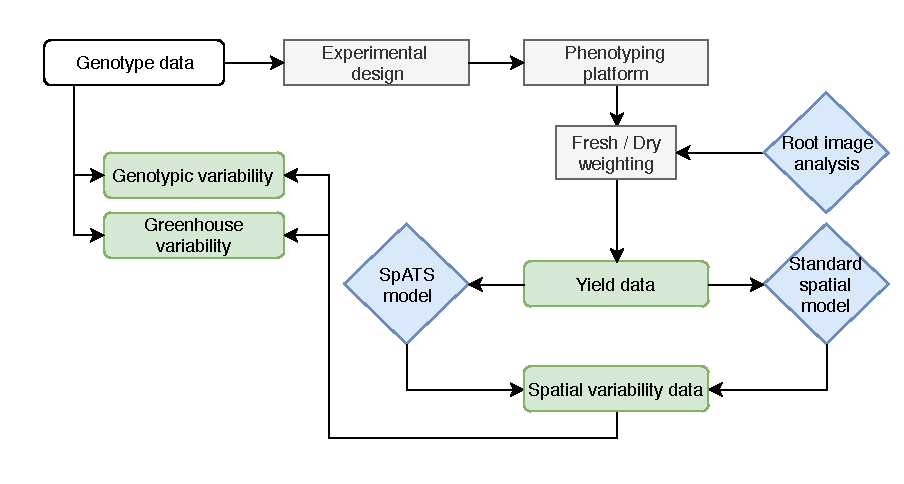
\includegraphics[width = \textwidth]{Pictures/methodology.pdf}
\end{frame}


\section{Platform}
\begin{frame}{Phenotyping platform}
Maize seeds are used - Germinated outside of the platform:
\begin{itemize}
    \item 2 tanks of 495 plants
    \item Root scan every 2 hours
    \item 1 tank moving 24/7, 1 tank still  
\end{itemize}
\begin{columns}
\begin{column}{0.5\textwidth}
\centering
\includegraphics[height = 4cm]{Pictures/root_platform.png}
\end{column}
\begin{column}{0.15\textwidth} 
\centering
\includegraphics[height = 5cm]{Pictures/root_scan.jpg}
\end{column}
\begin{column}{0.25\textwidth}
\centering
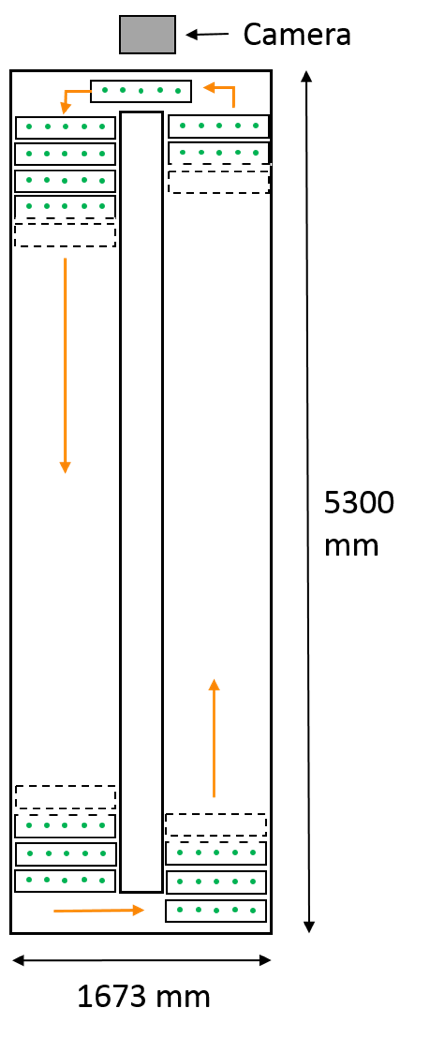
\includegraphics[height = 5.4cm]{Pictures/platform_tank_topview.png}
\end{column}
\end{columns}

\end{frame}
\section{Experimental Design}
\begin{frame}{Design factors}
\begin{columns}
\begin{column}{0.3\textwidth}
\centering
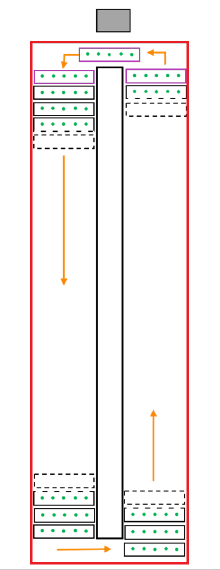
\includegraphics[height=6.8cm]{Pictures/factors.PNG}
\end{column}
\begin{column}{0.7\textwidth}
4 categorical factors:
\begin{itemize}
    \item \textcolor{red}{Tank}: 2 levels (moving or still)
    \item \textcolor{purple}{Strip}: 99 levels
    \item \textcolor{green}{Position} (on the strip): 5 levels
    \item Genotype: 30 levels
\end{itemize}~\\
Hierarchical order in the categories $\rightarrow$ creates \textit{blocking}:
\begin{itemize}
    \item 2 wholes plots $\approx$ 2 tanks
    \item 99 sub-plots $\approx$ 99 strips
\end{itemize}
\end{column}
\end{columns}
\end{frame}

\begin{frame}{Design output}
\centering
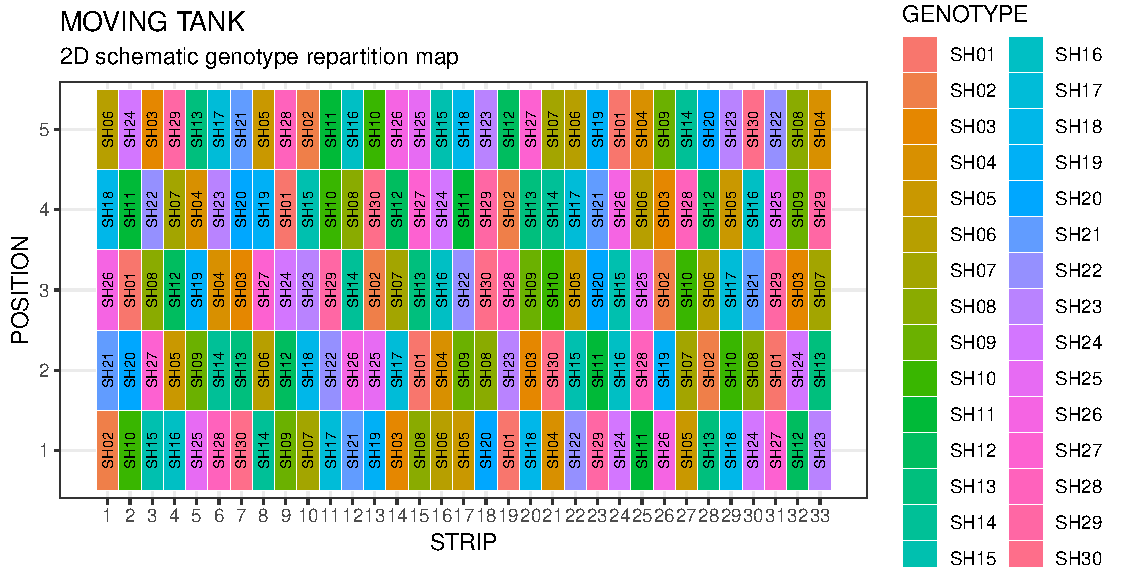
\includegraphics[width=\textwidth]{Pictures/moving_layout_30_genotypes.pdf}
\end{frame}

%%\section{Data processing}
%%\begin{frame}{Data processing pipeline}
%%Tracks root growth from root pictures
%%$\rightarrow$ Temporal component 
%%\begin{columns}
%%\begin{column}{0.5\textwidth}
%%Several indicators:
%%\begin{itemize}
%%    \item Number of root tips
%%    \item Total root length
%%    \item Growth speed
%%\end{itemize}
%%\end{column}
%%\begin{column}{0.5\textwidth} 
%%\centering
%%\includegraphics[width=4cm]{Pictures/root_tracking.png}
%%\end{column}
%%\end{columns}
%%Other interesting data from the plants: Dry/wet weight, leaf size, $\ldots$
%%\end{frame}

\section{Spatial models}

\begin{frame}{Spatial models}
Spatial models can be re-written as \textbf{mixed models}:
\[\mathbf{y}=\underbrace{\mathbf{X} \boldsymbol{\beta}}_{\substack{\text{Fixed}\\ \text{ effects}}}+\underbrace{\mathbf{Z} \mathbf{c}}_{\substack{\text{Random} \\ \text{ effects}}}+\underbrace{\boldsymbol{\xi}}_{\substack{\text{Spatially} \\ \text{dependant} \\ \text{error}}}+\underbrace{\boldsymbol{\varepsilon}}_{\substack{\text{Random}\\\text{error}}}\]
$\rightarrow$ Useful for \emph{variance estimation}.\\

With 2 kinds of effect:
\begin{itemize}
    \item \textbf{Fixed}: linked to environment (e.g. light distribution, slope)
    \item \textbf{Random}: cannot be linked to covariates (e.g. genotype effect, soil moisture) 
\end{itemize}

\end{frame}

\begin{frame}{Spatial variation}

Spatial variation in $\mathbf{y}$ can be decomposed in:
\begin{itemize}
    \item Global trends (stationary): rain, temperature ... %$\rightarrow$ fixed effects and row/col functions
    \item Local trends (non-stationary): patch of fertility, ... %$\rightarrow$ spatial error $\boldsymbol{\xi}$
    %Stationarity is a property of the random function model, not of the underlying spatial distribution%
    \item Extraneous variation: agricultural practices, ... %$\rightarrow$ fixed/random effects
\end{itemize}
~\\
2 main approaches to model this \emph{spatial variation}:
\begin{enumerate}
    \item Spatial variance-covariance structures
    \item Smoothing techniques
\end{enumerate}
\end{frame}

\begin{frame}{Standard spatial model (VCOV structure)}
Random ($\mathbf{c})$ and fixed ($\boldsymbol{\beta}$) effects modelled using covariates\\
Spatial error $\mathbf{e} = \boldsymbol{\xi} + \boldsymbol{\varepsilon}$ as a 2D random process
\begin{columns}
\begin{column}{0.5\textwidth}
\begin{itemize}
    \item Modelled using a \emph{semi-variogram}
    \item Equivalent to a $AR(1) \times AR(1)$ model
    ~\\ $\rightarrow$ only 2 parameters to estimate
    \item Elevated to a $LV \times LV$ model
    ~\\ $\rightarrow$ robust to convergence issues
\end{itemize}

\end{column}
\begin{column}{0.5\textwidth}
\centering
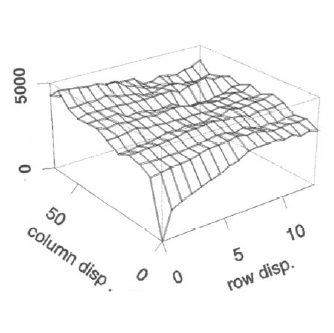
\includegraphics[width = 5.5cm]{Pictures/vario.PNG}
\end{column}
\end{columns}
\end{frame}


\begin{frame}{SpATS model (smoothing approach)}
Use of a \textbf{smooth bivariate surface} to model global trends \textbf{AND} local trends (no more spatial error term
$\boldsymbol{\xi}$)\\

$\rightarrow$ \emph{Linear} part, \emph{smooth} part and \emph{interactions}\\

\centering
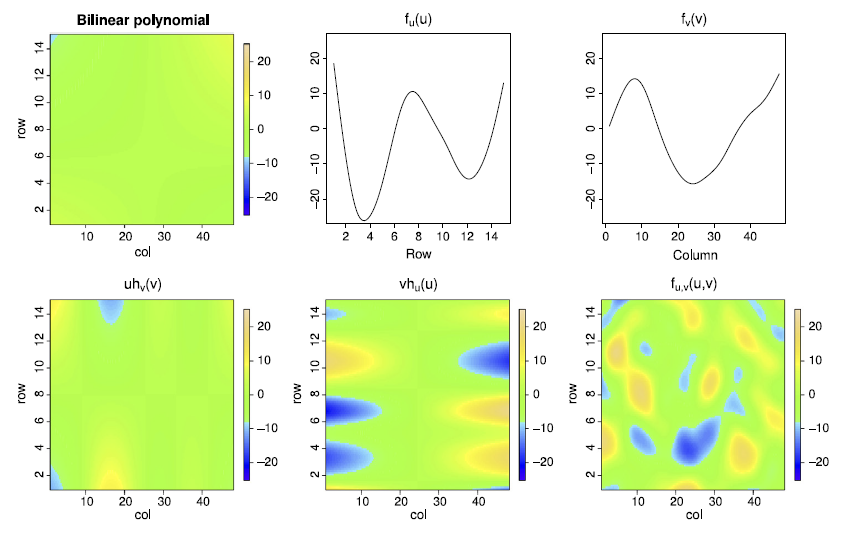
\includegraphics[height = 4.5cm]{Pictures/smoothing.PNG}
\end{frame}



%%\begin{frame}{Spatial models}
%%2 different models to estimate the spatial heterogeneity:
%%\begin{itemize}
%%    \item SpATS model: smooth bivariate surface along the rows and columns
%%    \item Linear variance model: product of linear variance along the rows and columns with an auto-regressive structure
%%\end{itemize}
%%    
%%\end{frame}
%%
%%\begin{frame}{SpATS model}
%%Spatial heterogeneity approximated by a \textit{smooth bivariate surface}:
%%\[\begin{aligned} f ( \boldsymbol { u } , \boldsymbol { v } ) = & \underbrace { \mathbf { 1 } _ { n } \beta _ { 0 } + \boldsymbol { u } \beta _ { 1 } + \boldsymbol { v } \beta _ { 2 } + \boldsymbol { u } \odot \boldsymbol { v } \beta _ { 3 } }_{ \text { Bilinear polynomial } } \\ & + \underbrace { f _ { u } ( \boldsymbol { u } ) + f _ { v } ( \boldsymbol { v } ) + \boldsymbol { u } \odot h _ { v } ( \boldsymbol { v } ) + \boldsymbol { v } \odot h _ { u } ( \boldsymbol { u } ) + f _ { u , v } ( \boldsymbol { u } , \boldsymbol { v } ) } _ { \text { Smooth part } } \end{aligned}\]
%%$f ( \boldsymbol { u } , \boldsymbol { v } )$ is modelled using tensor product of B-splines which can be rewritten as a mixed model:
%%\[y = \underbrace { X _ { s } \beta _ { s } + Z _ { s } c _ { s } } _ { f ( u , v ) } + \underbrace{X _ { d } \beta _ { d }}_{\text{Fixed effects}} + \underbrace{Z _ { d } c _ { d }}_{\text{Random effects}} + \quad \varepsilon \]
%%\end{frame}
%%
%%\begin{frame}{Linear Variance model}
%%Basic variance model with \emph{Baseline VCOV structure} ($V_0$) and \emph{Spatial correlation} ($V_S$):
%%\[V =V_{0}+V_{S}=\underbrace{\sigma^{2} I_{n}}_{\text{Nugget effect}}+\underbrace{\eta J_{n}}_{\text{Block effects}}+\underbrace{\phi M_{n}}_{\substack{\text{Spatial correlation with} \\\text{LV–covariance structure}}}\]
%%
%%The model can be augmented in 2D (LV$\otimes$LV) by using a product of the VCOV structure of the rows and columns:
%%\[V_{S}=\kappa V_{R} \otimes V_{C}\]
%%
%%\end{frame}

\section{Results}
\begin{frame}{Goal of the analysis}
4 questions to answer:
\begin{enumerate}
	\item Is there a significant difference between the \emph{moving} and \emph{still} tank ? 
	\item Do the models account for \emph{spatial trends} ?
	\item How different are the estimation of the two models ?
	\item Is there a significant \emph{genotypic effect}, picked up by the models ? 
\end{enumerate}
~\\
Using 4 variables:
\begin{itemize}
	\item \textbf{Fresh} weight for \textbf{root} and \textbf{leaf} system
	\item \textbf{Dry} weight for \textbf{root} and \textbf{leaf} system
\end{itemize}
\end{frame}

\begin{frame}{1. Tank difference}
\centering
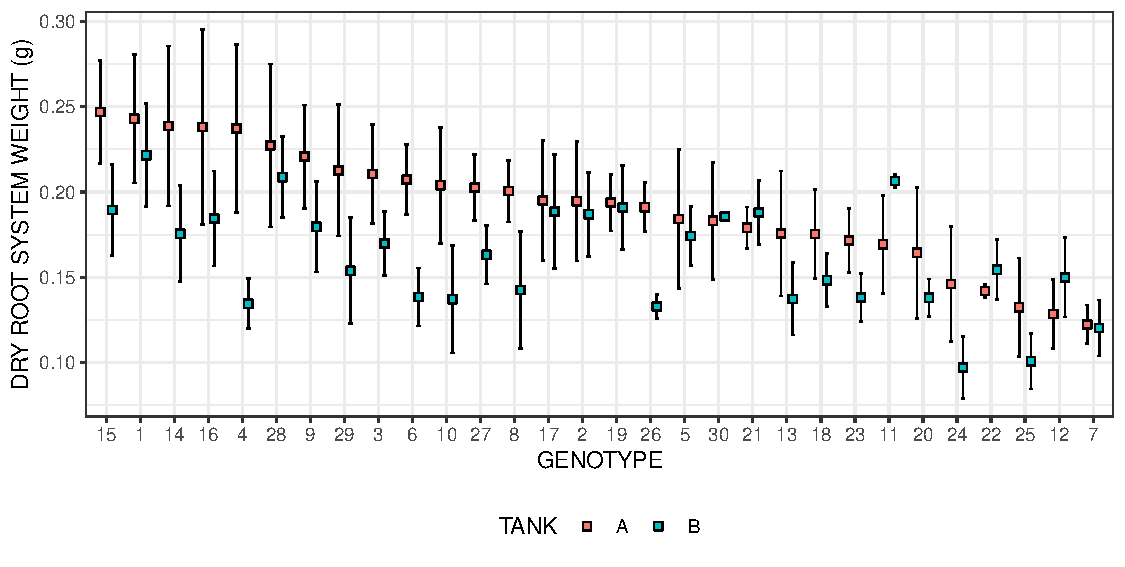
\includegraphics[height = 0.6\textheight]{Pictures/DRY_RS_summary_plot.pdf}
\begin{flushleft}
T-tests revealed significant difference between tanks $(p<0.05)$

$\rightarrow$ For all \emph{variables}

$\rightarrow$ \textbf{NOT} for all \emph{genotypes}
\end{flushleft}
\end{frame}

\begin{frame}{2. Model comparison}
\centering
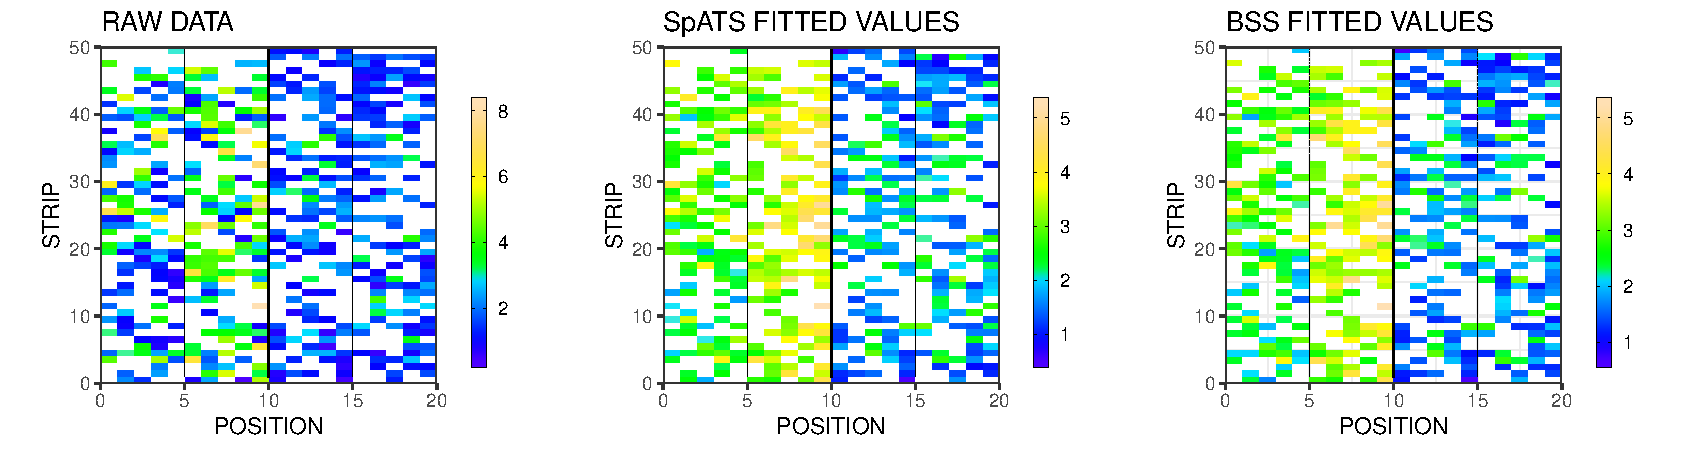
\includegraphics[width = \textwidth]{Pictures/model_comparison.pdf}
\flushleft
\begin{columns}
\begin{column}{0.6\textwidth}
Model outputs show:
\begin{itemize}
	\item Tank effect
	\item Highly similar values
	\item Clear spatial trends\\
	$\rightarrow$ mostly along the \textbf{STRIPS}\\
	$\rightarrow$ complex spatial patterns
\end{itemize}
\end{column}
\begin{column}{0.4\textwidth}
\danger  More heterogeneity in the \emph{moving tank}\\
$\rightarrow$ not picked up by the model
\end{column}
\end{columns}

\end{frame}

\begin{frame}{3. Genotypic effect}
\begin{columns}
	\begin{column}{0.6\textwidth}
	\begin{itemize}
		\item Models give \emph{similar values}
		\item Large part of the variation attributed to the genotypes\\
		$\rightarrow$ Significant genotypic effect
		\item Ranking similar to the weights
	\end{itemize}
	~\\
	 \danger Harder to interpret without context !
	\end{column}
	
	\begin{column}{0.4\textwidth}
	\centering
	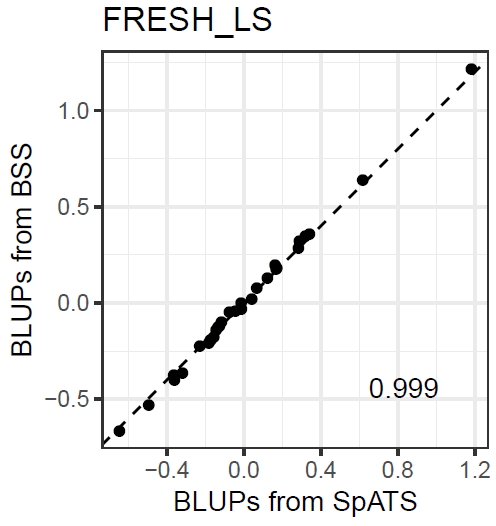
\includegraphics[width =4.5cm]{Pictures/GENO.PNG}
	\end{column}
\end{columns}
\end{frame}

\section{Conclusion}
\begin{frame}{Conclusion}
Main points:
\begin{itemize}
	\item Significant tank effect
	\item Strong genotypes differences
	\item Similar output for both models\\
	$\rightarrow$ Better interpretability for SpATS\\
	$\rightarrow$ No iterative process
	\item Clear spatial trends\\
	$\rightarrow$ Better captured in the \emph{still tank}
\end{itemize}
~\\
\begin{itemize}
	\item[?] Adapted to moving environment
	\item[?] Results of a less-complex GLM
	\item[?] Use of time dimension in the model
\end{itemize}

\end{frame}

\end{document}